% -*- TeX-master: "report" -*-

\section{Complex Predicates}
\label{sec-complex-preds}
This section gives a precise definition of complex predicates and discusses the trade-offs in our implementation.

A complex predicate $C$ is defined as $C = \phi(p_1, p_2, \ldots p_k)$ where $p_1, p_2, \ldots p_k$ are simple predicates and $\phi$ is a function that can be computed using only the logical operators $and$ and $or$.  The operator $not$ is not required because any propositional formula can be written in conjunctive normal form (CNF) in which the $not$ operator appears only before the literals.  By design, the negation of every simple predicate $P$ is also a predicate.

For a predicate $P$ and a run $R$, $R(P)$ = 1 if $P$ was observed to be true at least once during run $R$.  Similarly we could define $R(C)${\footnote{For sake of clarity, we use 1, 0 and $true, false$ interchangeably for the values of $R(C)$ and $R(P)$.}} as follows:
\begin{defn}
\label{dfn1}
For a complex predicate $C = \phi(p_1, p_2, \ldots p_k)$, $R(C)$ = 1 iff at some point during the execution of the program, $C$ was observed to be true.
\end{defn}

The difficulty with this notion of complex predicates is that $C$ must be explicitly monitored during the program execution.  For example, if $C_1 = p_1 \wedge p_2$ then $R(p_1)$ = 1 and $R(p_2)$ = 1 does not imply that $R(C)$ = 1.  $p_1$ and $p_2$ may be true at different stages of execution but never true at the same time.  However, as discussed earlier, explicitly monitoring $C$ requires significant changes to existing infrastructure.  In order to be able to estimate the value of $C$ from its components, we adapt a less precise definition as follows:
\begin{defn}
\label{dfn2}
For a complex predicate $C = \phi(p_1, p_2, \ldots p_k)$, $R(C)$ = 1 iff $\phi(R(p_1), R(p_2), \ldots R(p_k))$ = $true$
\end{defn}

In other words, we assume that $R$ is distributive over $\phi$.  This can lead to false positives, because $R(C)$ may be computed to 1 when it is actually 0, but no false negatives.  The impact of this assumption on the score of $C$ may be either positive or negative depending on whether $R$ failed or succeeded.

There are $2^{2^N}$ boolean functions of $N$ predicates ~\cite{MathWorld:BoolFuncs}.  This is a prohibitively large number considering that there can be hundreds of simple predicates.  To reduce the complexity, we consider only functions of two predicates.  There are $2^{2^2}$ = 16 such functions and their arguments can be chosen from $N$ predicates in $C^N_2 = \frac{N(N-1)}{2}$ ways.  Out of the 16 boolean functions of two variables, we consider only conjunction ($and$) and disjunction ($or$) since other functions are more complex and cannot be used effectively by the programmer.  Other functions can be easily included in our implementation once their truth tables (discussed in ~\autoref{sec-tvl}) are derived correctly.  To summarize, we evaluate only $2 \times C^N_2 = N(N-1)$ complex predicates.  If $R$ is the set of runs being analyzed then the time complexity required to build complex predicates is $|R|N(N-1) = O(|R|N^2)$

\subsection{Three valued logic}
\label{sec-tvl}
This section explains how conjunctions and disjunctions are actually computed.  Three-valued logic is used because the value of a predicate in a run may not be conclusive. This can arise in two situations:
\begin{enumerate}
\item The predicate was not observed in a run because the run did not reach the line where it was defined.
\item The program reached the line where the predicate was defined but was not observed because of sampling.
\end{enumerate}

In such a case, the value of a predicate $P$ is considered as $unknown$.  For the analysis introduced in ~\autoref{sec-bground}, it is enough to consider whether $R(P)$ was $true$ or $not\ true$ (both $false$ and $unknown$).  But while computing complex predicates, the two sub cases of the $not\ true$ case must be considered separately.

Consider a complex predicate $C = p_1 \wedge p_2$.  If either $p_1$ or $p_2$ was observed $false$ then $R(C) = false$.  If both $p_1$ and $p_2$ were observed $true$, then $C$ was observed to be true.  Otherwise, the value of $R(C)$ is $unknown$.  This is shown using a three-valued truth table in ~\autoref{tab:and}.

Similarly, for a complex predicate $D = p_1 \vee p_2$, if either $p_1$ or $p_2$ was observed $true$ then $R(D) = true$.  If both $p_1$ and $p_2$ were observed $false$, then $D$ was observed to be false.  Otherwise, the value of $R(D)$ is $unknown$.  This is shown using a three-valued truth table in ~\autoref{tab:or}.
 
\begin{table*}
\caption{3-valued Truth Table for $C = p_1 \wedge p_2$}
\label{tab:and}
\centering
\scriptsize
  
\begin{tabular}{c|ccc}
  % after \\: \hline or \cline{col1-col2} \cline{col3-col4} ...
  $P_1$$\backslash$$P_2$ & T & F & $?$ \\
  \hline
  T & T & F & ? \\
  F & F & F & F \\
  ? & ? & F & ? \\
\end{tabular}
\end{table*}


\begin{table*}
\caption{3-valued Truth Table for $D = p_1 \vee p_2$}
\label{tab:or}
\centering
\scriptsize
  
  \centering
  \begin{tabular}{c|ccc}
  % after \\: \hline or \cline{col1-col2} \cline{col3-col4} ...
  $P_1$$\backslash$$P_2$ & T & F & $?$ \\
  \hline
  T & T & T & T \\
  F & T & F & ? \\
  ? & T & ? & ? \\
\end{tabular}
\end{table*}

\subsection{Interesting Complex Predicate}

Even after imposing many constraints, the number of complex predicates is still quadratic in the number of simple predicates.  A large number of complex predicates formed by this procedure are likely to be useless in the analysis of the program.  A complex predicate that has a lower score than one of its components is useless.  The component (simple) predicate with a higher score is a better predictor of failure, and so the complex predicate adds nothing to the analysis.

\begin{defn}
\label{dfn3}
A complex predicate $C = \phi(p_1, p_2, \ldots p_k)$ is ``interesting'' iff $Importance(C) > Importance(p_i)$ for all $i \in \{1, 2, \ldots k\}$
\end{defn}

In the case where the complex predicate has the same score as the component predictor with higher score, the simpler one is preferable.  Keeping only interesting combinations of predicates reduces the memory burden of storing them, and helps ensure the utility of a complex predicate that is presented to the user.  Definition ~\ref{dfn3} is for the general case and as explained earlier, we explore only the case where $k = 2$ and $\phi \in \{\vee, \wedge\}$.

\subsection{Pruning}
\label{sec-pruning}
Forming a complex predicate from its components is a nontrivial task, requiring a conjunction or disjunction for each program run.  After this computation is complete the score of the newly formed predicate can be calculated, potentially labeling it uninteresting.  In such a case the effort to form the predicate has been wasted.  This provides the motivation to prune combinations early based on an estimate of their resulting scores.  An upper bound for a predicate's score can be determined by maximizing $F(P)$ and $Increase$ under constraints based on the propositional operation.  The score of the predicate (Eqn. ~\ref{eqn2}), being a harmonic mean of these two terms, will likewise be maximized.

In this context, the disjunction $D = p_1 \vee p_2$ can be considered as the union of the set of runs where $p_1$ was $true$ and the set where $p_2$ was $true$.  The size of the resulting set is maximized when the two do not overlap, and that is the assumption made when calculating an upper bound on $F(D)$.  $S(D)$ is minimized by making the opposite assumption - that one is a subset of the other.  The size of the union is thus the size of the superset.  The best disjunction that can be formed using $p_1$ and $p_2$ will have the following parameters:

\begin{eqnarray*}
  F(D)' &=&  F(p_1) + F(p_2) \\
  S(D)' &=&  \max(S(p_1),S(p_2)) \\
  F(D\;observed)' &=& 0 \\
  S(D\;observed)' &=& S(D)'
\end{eqnarray*}

The second term in $Increase$ (Eqn. ~\ref{eqn1}) can only reduce the result, and so it is ignored in calculating an upper bound.  For completeness, $S$($D$ observed)$'$ is assigned the same value as $S(D)'$ even though it does not affect $Increase(D)$.  The $F(D)$ component of $Importance$ is maximized while maximizing $Increase$.  Thus the $Importance$ score calculated with the above values is an upper bound on the score of the disjunction of $p_1$ and $p_2$.

The conjunction $C = p_1 \wedge p_2$ can be regarded as the intersection of the set of runs where $p_1$ was $true$ and the set where $p_2$ was $true$.  Maximizing $F(C)$ requires that one of the intersecting sets is a subset of the other, making the size of the intersection the size of the smaller set.  A minimal $S(C)$ is found when the component sets are non overlapping; the intersection of two such sets is empty.

\begin{eqnarray*}
  F(C)' &=&  \min(F(p_1),F(p_2)) \\
  S(C)' &=& 0
\end{eqnarray*}

If the second term in $Increase$ is ignored, as with disjunctions, the upper bound of a conjoined predicate's $Increase$ score is 1.  This is the maximum $Increase$ possible, reducing the likelihood of a conjoined predicate being pruned to almost zero.  The second term is therefore used for conjunctions to drop the upper bound to a more useful level.

$F(C$ observed) is minimized by assuming that $C$ was \textit{observed} only in the (failed) runs where it was true.  Maximizing $S(C$ observed) is more difficult.  Recall that a conjunction can be considered \textit{observed} if either component is \textit{observed false}, or both are \textit{observed true}.  The combination of successful runs where a predicate is \textit{observed false} (union) is maximized if the sets are non overlapping, while the combination where they are \textit{observed true} (intersection) is maximized if one is a subset of the other.  By assuming both cases meet that criteria $S(C$ observed) can be maximized.  Its value is the sum of successful runs where $p_1$ was \textit{observed} and those where $p_2$ was \textit{observed false}, formed as the difference between $S(p_2$  Observed) and $S(p_2)$. Figure \ref{maxsuccess} depicts the above scenario: notice that the sets $S(\neg p_1)$ and $S(\neg p_2)$ are disjoint and $s(p_1)$ is a subset of $s(p_2)$.  Since the result may differ depending on which predicate is chosen as $p_1$ the larger result is used.
\begin{eqnarray*}
  F(C\;obs)' &=& F(C)' \\
  S(C\;obs)' &=&
  \max(S(p_1\;obs)+S(p_2\;obs)-S(p_2),\\
  & &\ \ \ \ S(p_2\;obs)+S(p_1\;obs)-S(p_1))
\end{eqnarray*}

\begin{figure}[h]
  \centering
  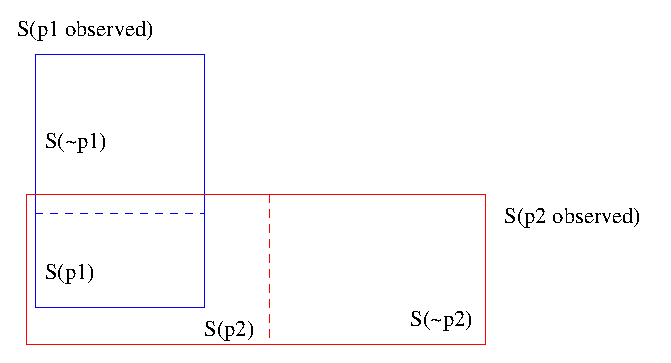
\includegraphics[scale = 0.6]{charts/maxsuccess}  
  \caption{Maximizing S(C observed)}
  \label{maxsuccess}
\end{figure}


Pruning is useful when a computed complex predicate, $C = \phi(p_1, p_2)$, will be thrown away if its score falls below a threshold.  Such a threshold can be found in two ways:
\begin{enumerate}
\item The scores of $p_1$ and $p_2$ that determine whether $C$ is interesting or not.
% Changed 'lowest' to 'highest', because a complex pred must beat the
% best known pred to be considered, not the worst known.
\item During the redundancy elimination, the highest % just thought about it... our implementation does not do this
score among simple predicates can be used as the threshold because if the score is below this value, computing $C$ is useless for this iteration.
\end{enumerate}
